\documentclass[a4paper,11pt]{ltjsarticle}
\usepackage{graphicx}
\usepackage{booktabs}
\usepackage{amsmath}
\usepackage{siunitx}
\usepackage[margin=22mm]{geometry}
\usepackage{caption}
\usepackage{placeins}
\usepackage[hidelinks]{hyperref}
\captionsetup{font=small,labelfont=bf}
\newcommand{\best}[1]{\textbf{#1}}

\title{トポロジー最適化の結果を\\オーバーハングのない形に直す生成モデル\\[0.4em]\large これまでの検討のまとめ}
\date{2026年10月23日}

\begin{document}
\maketitle

\section{目的}

積層造形（AM）では，造形方向に対して張り出しの大きい部分（オーバーハング）はサポートがないと造れない．
普通のトポロジー最適化の結果はオーバーハングを考慮していないので，そのままではサポートが必要になる．
オーバーハング制約付きのトポロジー最適化を解けば自己支持の形が得られるが，条件ごとに最適化を解き直す必要がある．

そこで，普通のトポロジー最適化の結果と条件（拘束・荷重・体積率・造形方向）を入力すると，
サポートなしで造れる形（張り出しは造形方向から \ang{45} まで）を出力する生成モデルを作る．
生成モデルを使うと，同じ入力から複数の案を作り，有限要素解析で一番良い案を選ぶこともできる．

\section{手法}

\subsection{問題設定}

設計領域は $64 \times 32$ 要素の 2 次元弾性体（四角形 1 次要素，要素寸法 1）とする．
造形方向は上向き（下端がベースプレート）とし，オーバーハングの限界角は \ang{45} とする．
目的関数はコンプライアンス，制約は体積率である．

\subsection{教師データの作り方}

教師データの組は JuliaOptopus で作る．1 件ごとに，同じ条件で次の 2 つを解く．
\begin{itemize}
  \item \textbf{入力（free）}：AM の制約なしのトポロジー最適化．
  \item \textbf{正解（self）}：Langelaar のサポート共最適化で，サポートを禁止したもの（自己支持の材料だけで造れる形）．
\end{itemize}
どちらも密度フィルター（半径 $r = 1.5h$），Heaviside 射影（$\beta = 5$），SIMP（$p = 3$），MMA で，最大 100 反復解く．

条件は次のように乱数で作る．
\begin{itemize}
  \item 支え方：片持ち梁（左端を固定），両端固定，ピンとローラー（下端の両隅）から 1 つ．
  \item 荷重：境界上の 2〜3 節点にかかる線荷重 1 つ．合計の大きさは 1，向きは乱数で決める．
  \item 体積率：0.3〜0.5 の一様乱数．
\end{itemize}

\subsection{モデルの入力と出力}

入力は 7 チャネルの画像（$32 \times 64$）である．
内訳は，free の密度，体積率（一定値の画像），$x$・$y$ 方向の拘束，$x$・$y$ 方向の荷重，ベースプレートの位置（造形方向を表す）である．
出力は 1 チャネルの密度である．
体積率のチャネルは，入力の密度から読み取れるので要らない可能性がある．
外して学習した結果は，どの指標もほぼ同じだった（\ref{sec:first} 節）．

\subsection{生成モデル}

どちらのモデルも，同じ U-Net（PhysicsNeMo の TopoDiff の U-Net，約 1070 万パラメータ）を使う．
\begin{itemize}
  \item \textbf{拡散モデル}：DDPM で学習し（cosine スケジュール，$T = 1000$），DDIM の 50 ステップで生成する．
  \item \textbf{フローマッチング}：rectified flow で学習し，Euler 法の 20 ステップで生成する．
        生成のステップが少ないので，拡散モデルより約 2.5 倍速い．
\end{itemize}
学習はどちらも 200 エポック，バッチ 32，学習率 $2 \times 10^{-4}$，EMA 0.999 とし，検証の損失が最小のエポックのモデルを使う．

\subsection{評価の指標}

テストの各条件について 4 案を生成し，主に 1 案目で評価する．
\begin{itemize}
  \item \textbf{コンプライアンスの比}：生成した形のコンプライアンス ÷ 正解のコンプライアンス（Python の有限要素解析で計算）．1 に近いほど良い．
  \item \textbf{造れない材料}：0.5 で白黒にした形で，ベースプレートから \ang{45} 以内の支えをたどれない材料．
        その割合が 0 でない案と，材料の 1\% を超える案の割合を示す．
  \item \textbf{浮いた材料}：ベースプレートにつながっていない材料．
  \item \textbf{IoU}：正解との形の一致度（0.5 で白黒にして計算）．
  \item \textbf{4 案から選んだ比}：4 案のうち，コンプライアンスが一番小さい案の比．
\end{itemize}

\section{データセット}

\subsection{最初のデータセット（5000 件）}

上の方法で 5000 件（学習 4250 件，検証 250 件，テスト 500 件）のデータを作った．
14 コアの Mac で 12 プロセスを並列に動かし，1 件あたり数秒〜20 秒程度で解ける．
図~\ref{fig:data} にデータの例を示す．

入力（free）には，95\% の件に造れない材料がある（材料の平均 25\%）．
正解（self）ではそれがほぼ 0 になり，コンプライアンスの増加は中央値で 2\% である．
ただし，正解には細い部材と中間の密度（グレー）が多く残る．
グレーの割合（材料のうち密度が 0.1〜0.9 の部分の割合）の中央値は 0.15 だった．

\begin{figure}[tb]
  \centering
  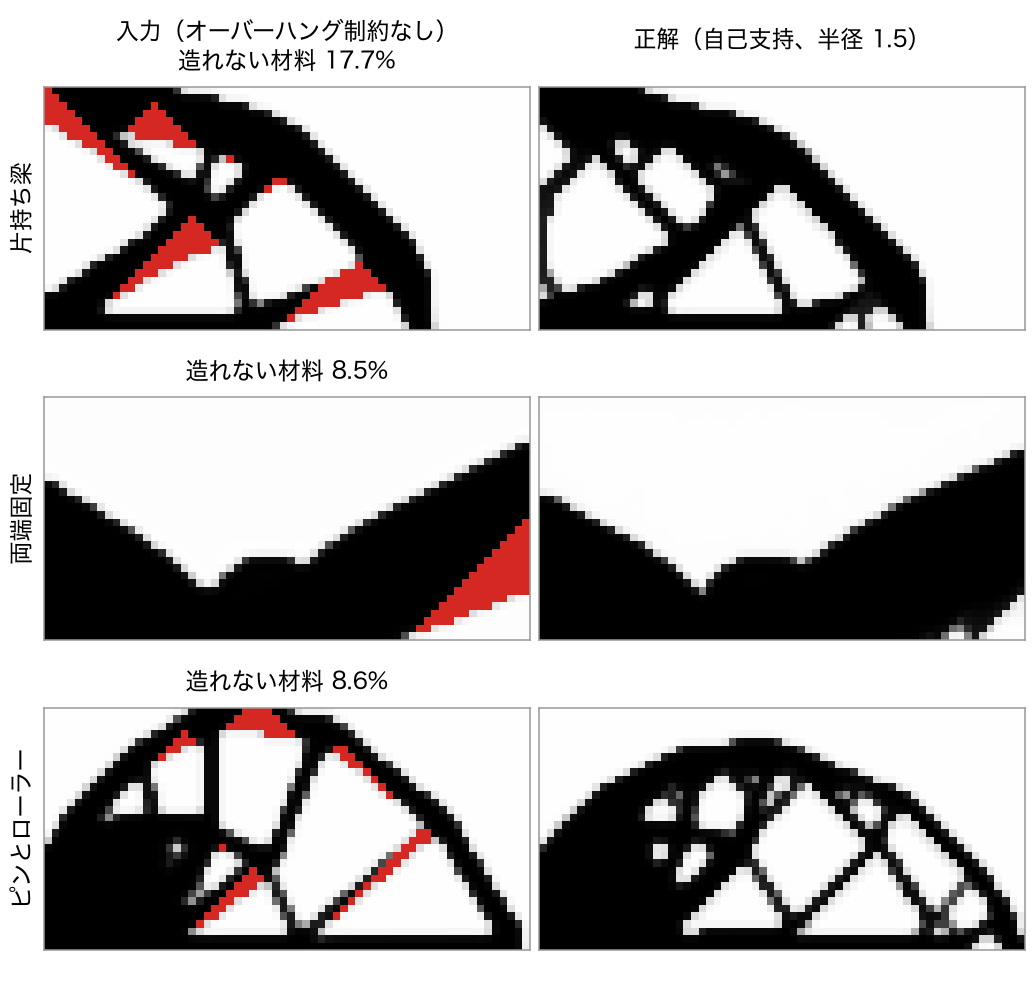
\includegraphics[width=0.62\linewidth]{figs/fig_data.png}
  \caption{最初のデータセットの例．赤は下に支えがなく造れない材料．}
  \label{fig:data}
\end{figure}

\subsection{単純化したデータセット（4799 件）}

細い部材とグレーを減らすために，正解（self）を次の設定で解き直した（\ref{sec:simplify} 節）．
入力（free）は変えていない．
\begin{itemize}
  \item 密度フィルターの半径を $1.5h$ から $4h$ に広げる．
  \item 射影の $\beta$ を 60 反復目から 30 反復ごとに $5 \to 8 \to 12 \to 16 \to 24 \to 32$ と上げる（$\beta$ の継続法）．
  \item 最大 350 反復解く．
\end{itemize}
解き直した後，グレーの割合が 0.15 を超える 201 件（片持ち梁 118 件，ピンとローラー 81 件，両端固定 2 件）を外した．
残った正解は 0.5 で白黒にした．
件数は 4799 件（学習 4049 件，検証 250 件，テスト 500 件）である．
表~\ref{tab:simplify} に，元の正解と比べた値を示す．

\begin{table}[tb]
  \centering
  \caption{元の正解と単純化した正解（5000 件）}
  \label{tab:simplify}
  \begin{tabular}{lcc}
    \toprule
    項目 & 元の正解 & 単純化した正解 \\
    \midrule
    フィルター半径・射影の $\beta$ & $1.5h$・5 & $4h$・$5 \to 32$ \\
    グレーの割合（中央値／95\% 点） & 0.142／0.376 & 0.021／0.132 \\
    穴の数（白黒にして数える．中央値／90\% 点） & 3／11 & 1／5 \\
    コンプライアンスの比（単純化 ÷ 元，中央値） & --- & 0.996 \\
    0.5 で白黒にしたときのコンプライアンスの比（中央値／最大） & --- & 0.999／1.014 \\
    造れない材料がある正解 & ほぼ 0 & 0.1\% \\
    \bottomrule
  \end{tabular}
\end{table}

\section{結果}

\subsection{最初のデータセットでの結果}
\label{sec:first}

最初のデータセット（5000 件）で拡散モデルを学習した．
結果を表~\ref{tab:first} に，生成した形の例を図~\ref{fig:first} に示す．
評価には，テストのうち番号 2000 以降の 291 件を使った（後の比較でも同じ件を使う）．

\begin{table}[tb]
  \centering
  \caption{最初のデータセット（5000 件）で学習した拡散モデル（テスト 291 件）}
  \label{tab:first}
  \begin{tabular}{lcc}
    \toprule
    指標 & 入力 & 拡散モデル \\
    \midrule
    造れない材料がある案 & 95\% & 18\% \\
    \quad うち材料の 1\% を超える案 & --- & 5\% \\
    造れない材料の割合（平均） & 25.0\% & 0.30\% \\
    浮いた材料がある案（材料の 1\% を超える案） & --- & 35\%（11\%） \\
    IoU（中央値） & 0.71 & 0.78 \\
    コンプライアンスの比（中央値） & 0.98 & 1.024 \\
    \quad 1.05 以下の案／2 倍を超える案 & --- & 78\%／1\% \\
    4 案から選んだ比（中央値） & --- & 1.007 \\
    \bottomrule
  \end{tabular}
\end{table}

\begin{figure}[tb]
  \centering
  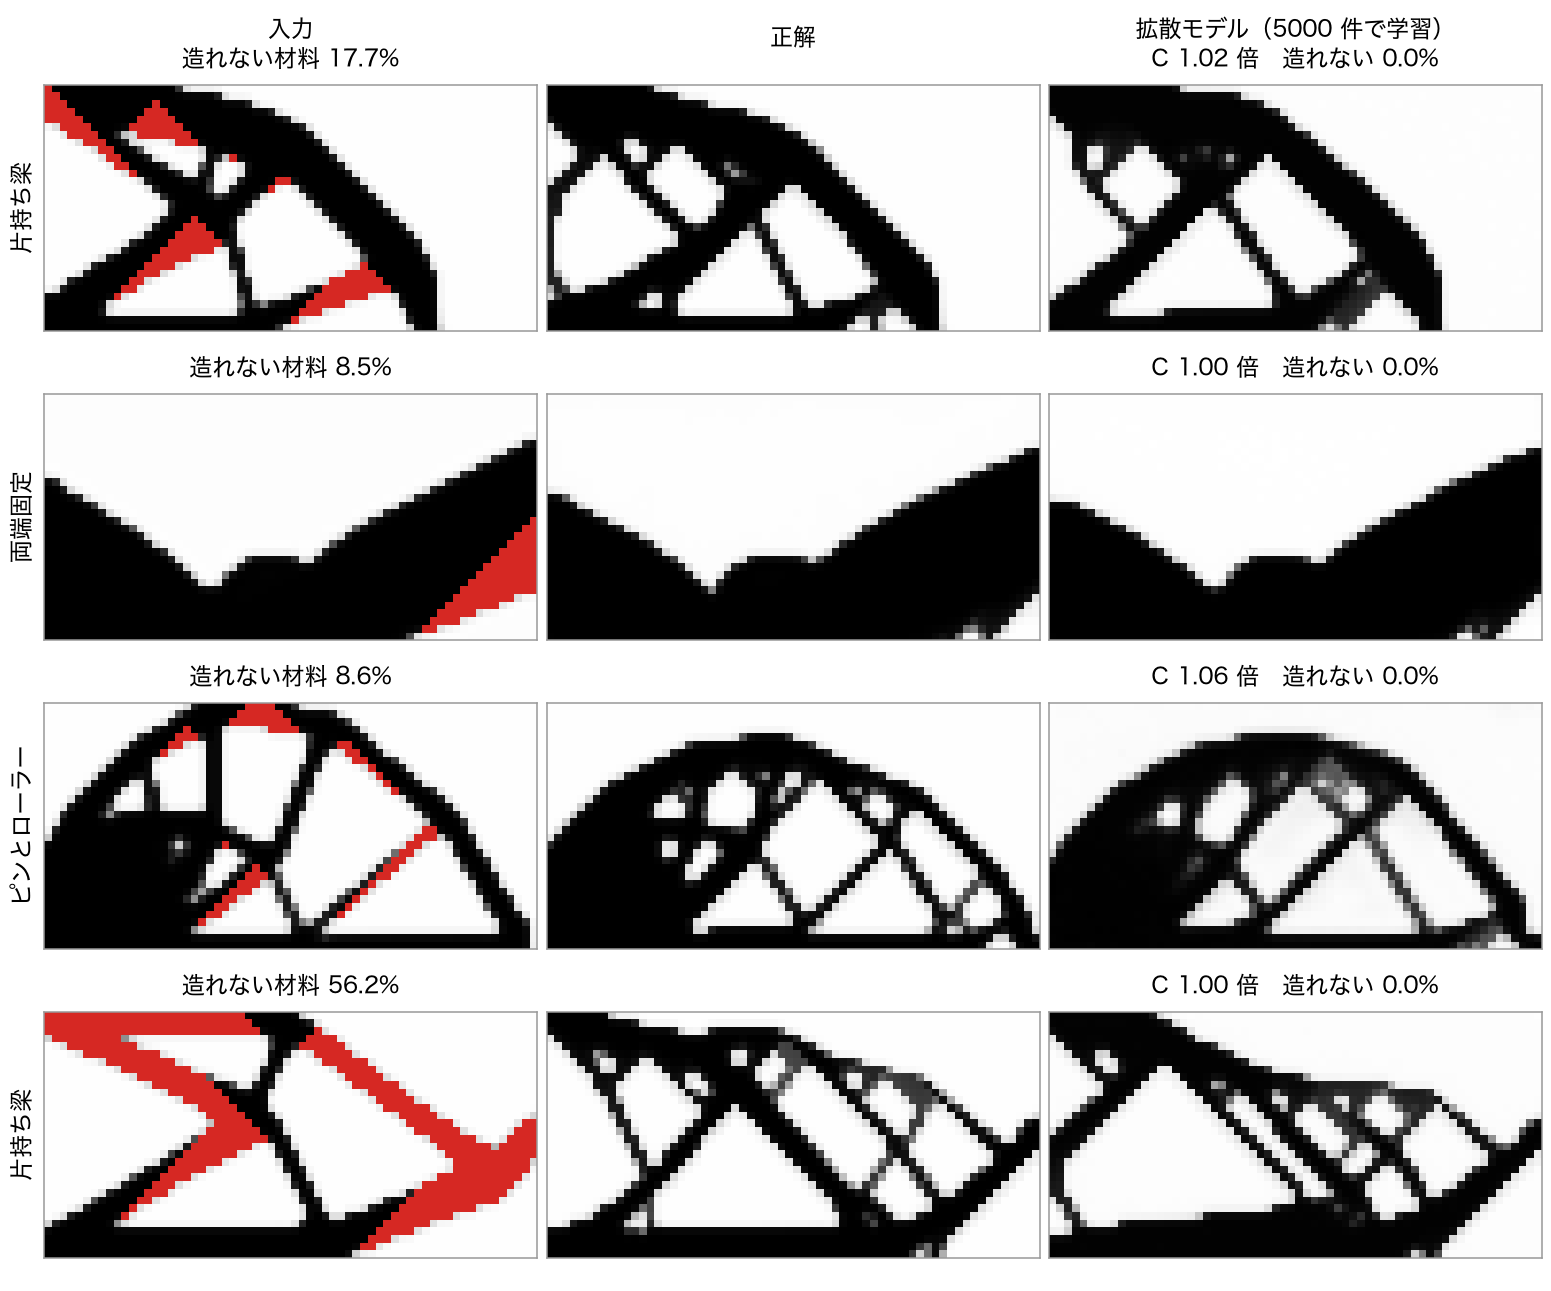
\includegraphics[width=0.85\linewidth]{figs/fig_first.png}
  \caption{最初のデータセット（5000 件）で学習した拡散モデルの出力（1 案目）．
           C は正解に対するコンプライアンスの比．赤は造れない材料．}
  \label{fig:first}
\end{figure}

5000 件で学習すると，正解の複雑な骨組み（細い部材や小さな穴）までおおむね再現できた．
造れない材料は，入力の平均 25\% から 0.30\% に減った．
コンプライアンスの比の中央値は 1.024，4 案から選べば 1.007 である．
一方，浮いた材料のある案が 35\% あった．
その多くは材料の 1\% 以下の小さなかけらである．

同じデータで，体積率を入力から外した拡散モデルと，フローマッチングも学習した．
体積率を外しても，どの指標もほぼ同じだった（コンプライアンスの比 1.026，造れない材料がある案 21\%）．
フローマッチングは，IoU 0.79，コンプライアンスの比 1.018 と拡散モデルに近い値だった．
ただし，造れない材料がある案は 26\% で，拡散モデルの 18\% より多かった．

\subsection{グレーの問題と正解の白黒化}

5000 件で学習したモデルの出力には，正解と同じくらいのグレーが残った．
出力のグレーの割合は中央値 0.17 で，正解の 0.16 とほぼ同じである．
モデルは正解のグレーまで学習していた．

そこで，正解を 0.5 で白黒にして学習し直した（入力はそのまま）．
出力のグレーの割合は 0 になった（図~\ref{fig:binarize}）．
しかし，形の複雑さは変わらなかった．
穴の数の平均は，グレーありのモデルが 4.4，白黒のモデルが 4.4 である．
造れない材料がある案は，拡散モデルで 18\% から 24\% に，フローマッチングで 26\% から 36\% に増えた．
グレーで表されていた細い部材が白黒の細い部材になり，途切れやすくなったためと考えられる．
正解の細い部材は製造の面でも難しいので，正解そのものを単純にすることにした．

\begin{figure}[tb]
  \centering
  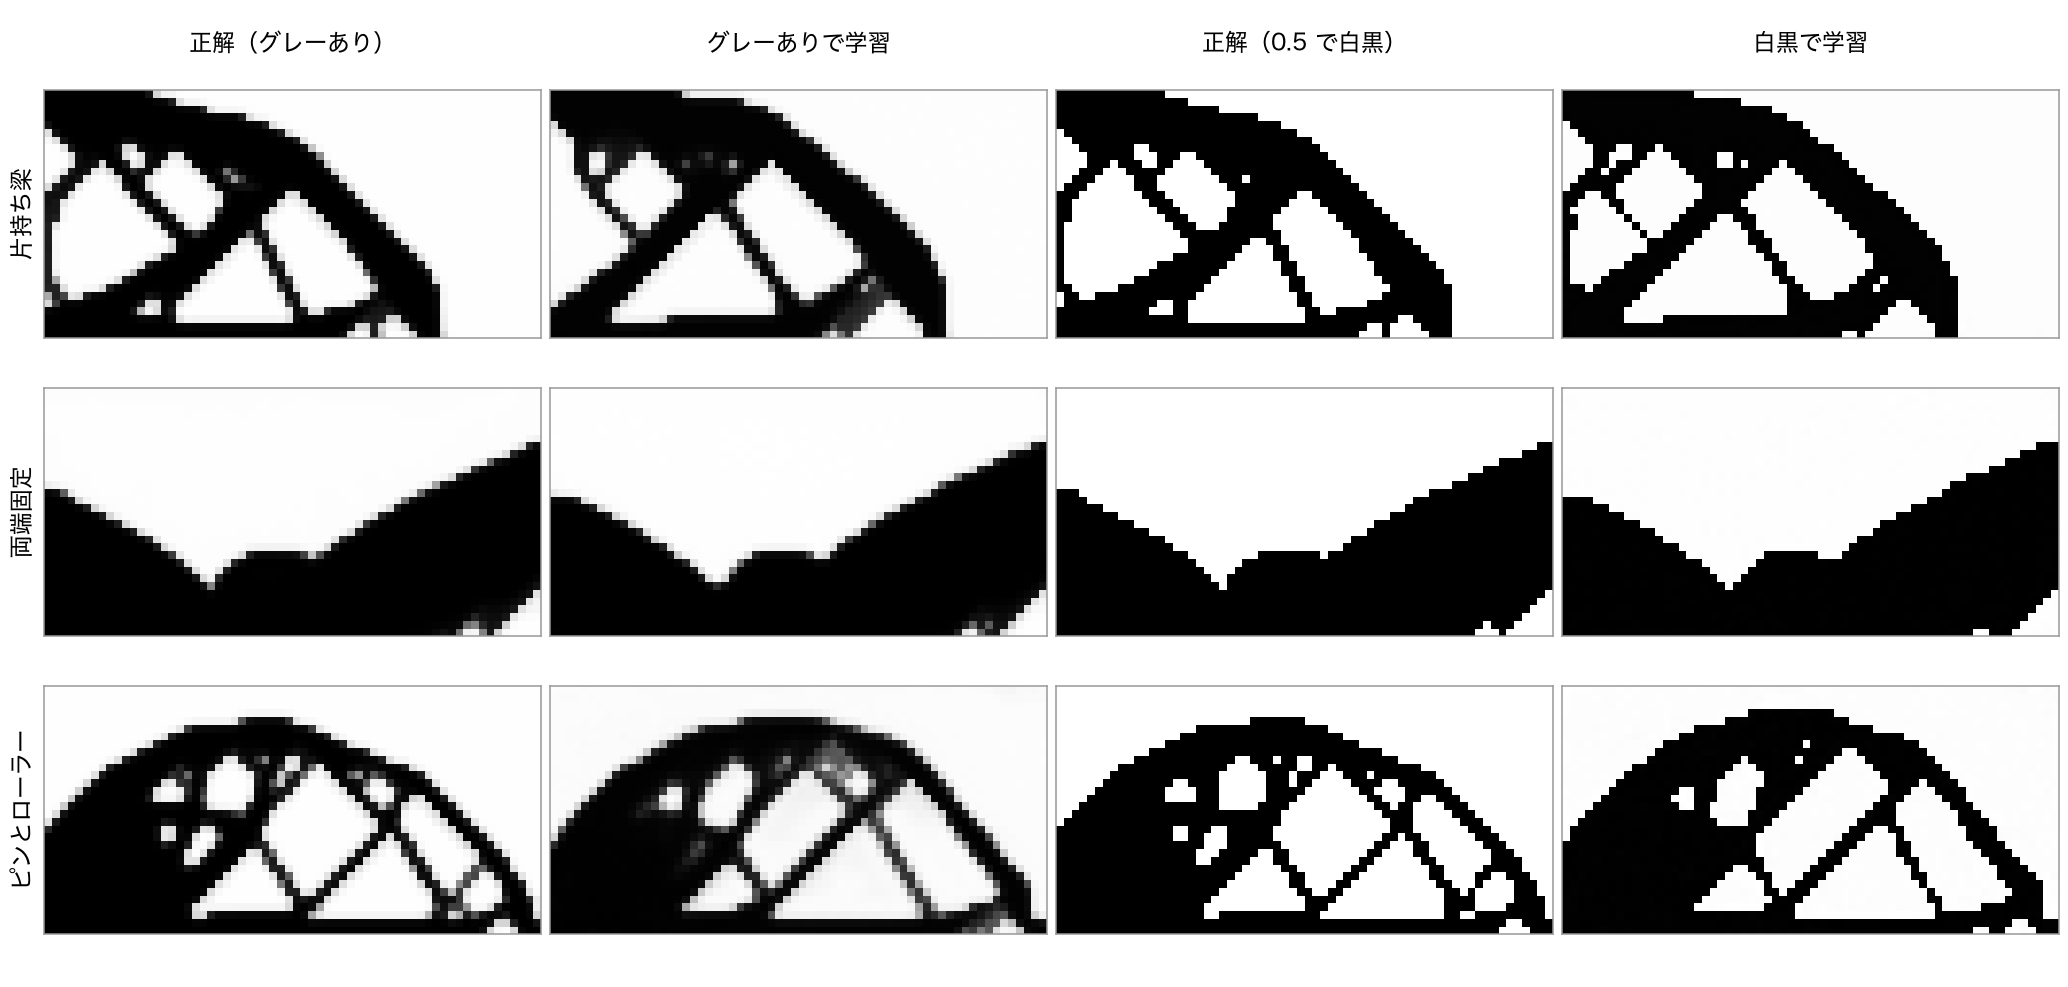
\includegraphics[width=0.85\linewidth]{figs/fig_binarize.png}
  \caption{正解を白黒にした効果（拡散モデル，5000 件）．出力からグレーは消えるが，細い部材は残る．}
  \label{fig:binarize}
\end{figure}

\FloatBarrier
\subsection{正解の単純化}
\label{sec:simplify}

「構造を単純にし，オーバーハング制約は満たす」正解を作るために，次の方法を 10 件（うちトラス状の 5 件）で試した．
\begin{enumerate}
  \item \textbf{最小部材寸法の幾何制約}（Zhou ら，2015）：元の正解を初期値にして，制約付きで最適化を続けた．
        細い部材は消えたが，細かいトラスの 4 件に 1 件で荷重の通り道が切れた．
  \item \textbf{穴の数の制約}（なめらかなオイラー標数）：穴に薄いグレーの膜を張る，部材を切り離す，などで制約をすり抜けた．
        白黒にして数えた穴は，ほとんど減らなかった．
  \item \textbf{穴の数の罰則}（永続ホモロジー）：白黒にして数えた穴は本当に減った（21 個から 11 個など）．
        ただし，埋めた穴や取り除いた部材が，しきい値ぎりぎりのグレーで残った．
  \item \textbf{大きなフィルター半径と $\beta$ の継続法}：self を一様な初期値から解き直した．\textbf{これを採用した．}
\end{enumerate}

4 の方法では，フィルター半径を大きくすると細い部材ができにくくなり，形が単純になる．
ただし，半径を大きくするとグレーが増える．
そこで，射影の $\beta$ を段階的に 32 まで上げてグレーを消した．
最初から $\beta = 32$ にすると，形が崩れた．
図~\ref{fig:simplify} に元の正解と単純化した正解を示す．
部材が太くなり，穴が減っている．
コンプライアンスはほとんど変わらない（表~\ref{tab:simplify}）．

\begin{figure}[tb]
  \centering
  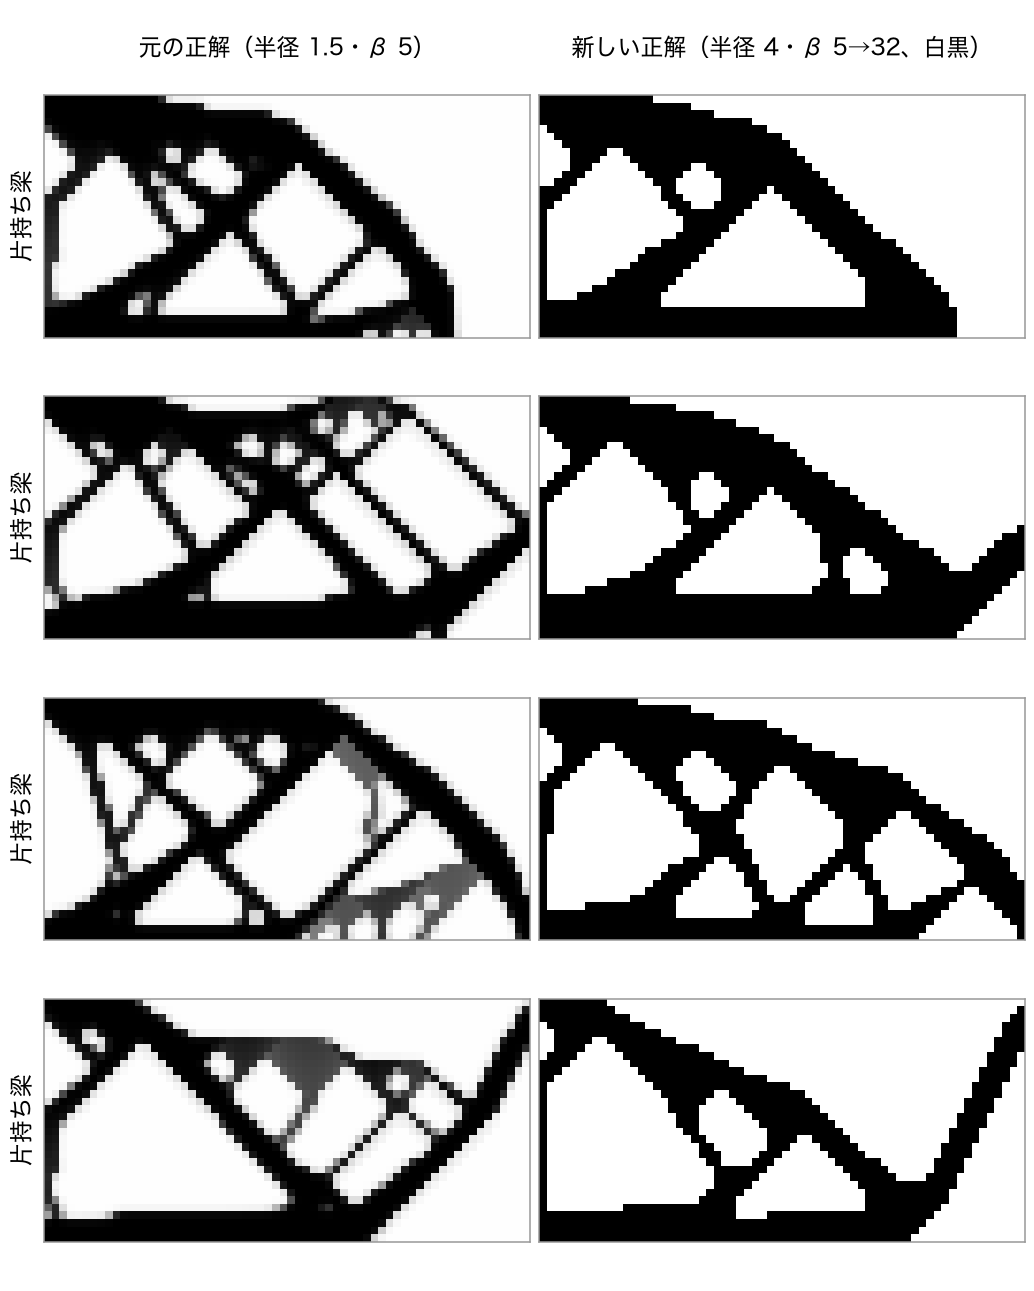
\includegraphics[width=0.62\linewidth]{figs/fig_simplify.png}
  \caption{元の正解（左）と単純化した正解（右）．}
  \label{fig:simplify}
\end{figure}

\subsection{単純化した正解での結果}

単純化したデータセット（4799 件）で，拡散モデルとフローマッチングを同じ設定で学習した．
2 つを並行に学習して，それぞれ 179 分かかった．
テスト 500 件の結果を表~\ref{tab:final} に，生成した形の例を図~\ref{fig:results} に示す．

\begin{table}[tb]
  \centering
  \caption{単純化した正解で学習したモデル（テスト 500 件）}
  \label{tab:final}
  \begin{tabular}{lcc}
    \toprule
    指標 & フローマッチング & 拡散モデル \\
    \midrule
    生成のステップ数 & 20 & 50 \\
    IoU（中央値） & \best{0.893} & 0.852 \\
    コンプライアンスの比（中央値） & \best{1.011} & 1.026 \\
    \quad 1.05 以下の案／2 倍を超える案 & \best{85\%／2\%} & 78\%／3\% \\
    4 案から選んだ比（中央値） & \best{1.001} & 1.009 \\
    造れない材料がある案（入力では 97\%） & 12\% & 9\% \\
    \quad うち材料の 1\% を超える案 & \best{3\%} & 5\% \\
    浮いた材料がある案（材料の 1\% を超える案） & 3\%（0\%） & 4\%（0\%） \\
    グレーの割合（中央値） & 0 & 0 \\
    穴の数の平均（正解は 1.63） & 1.70 & 1.66 \\
    \bottomrule
  \end{tabular}
\end{table}

\begin{figure}[tb]
  \centering
  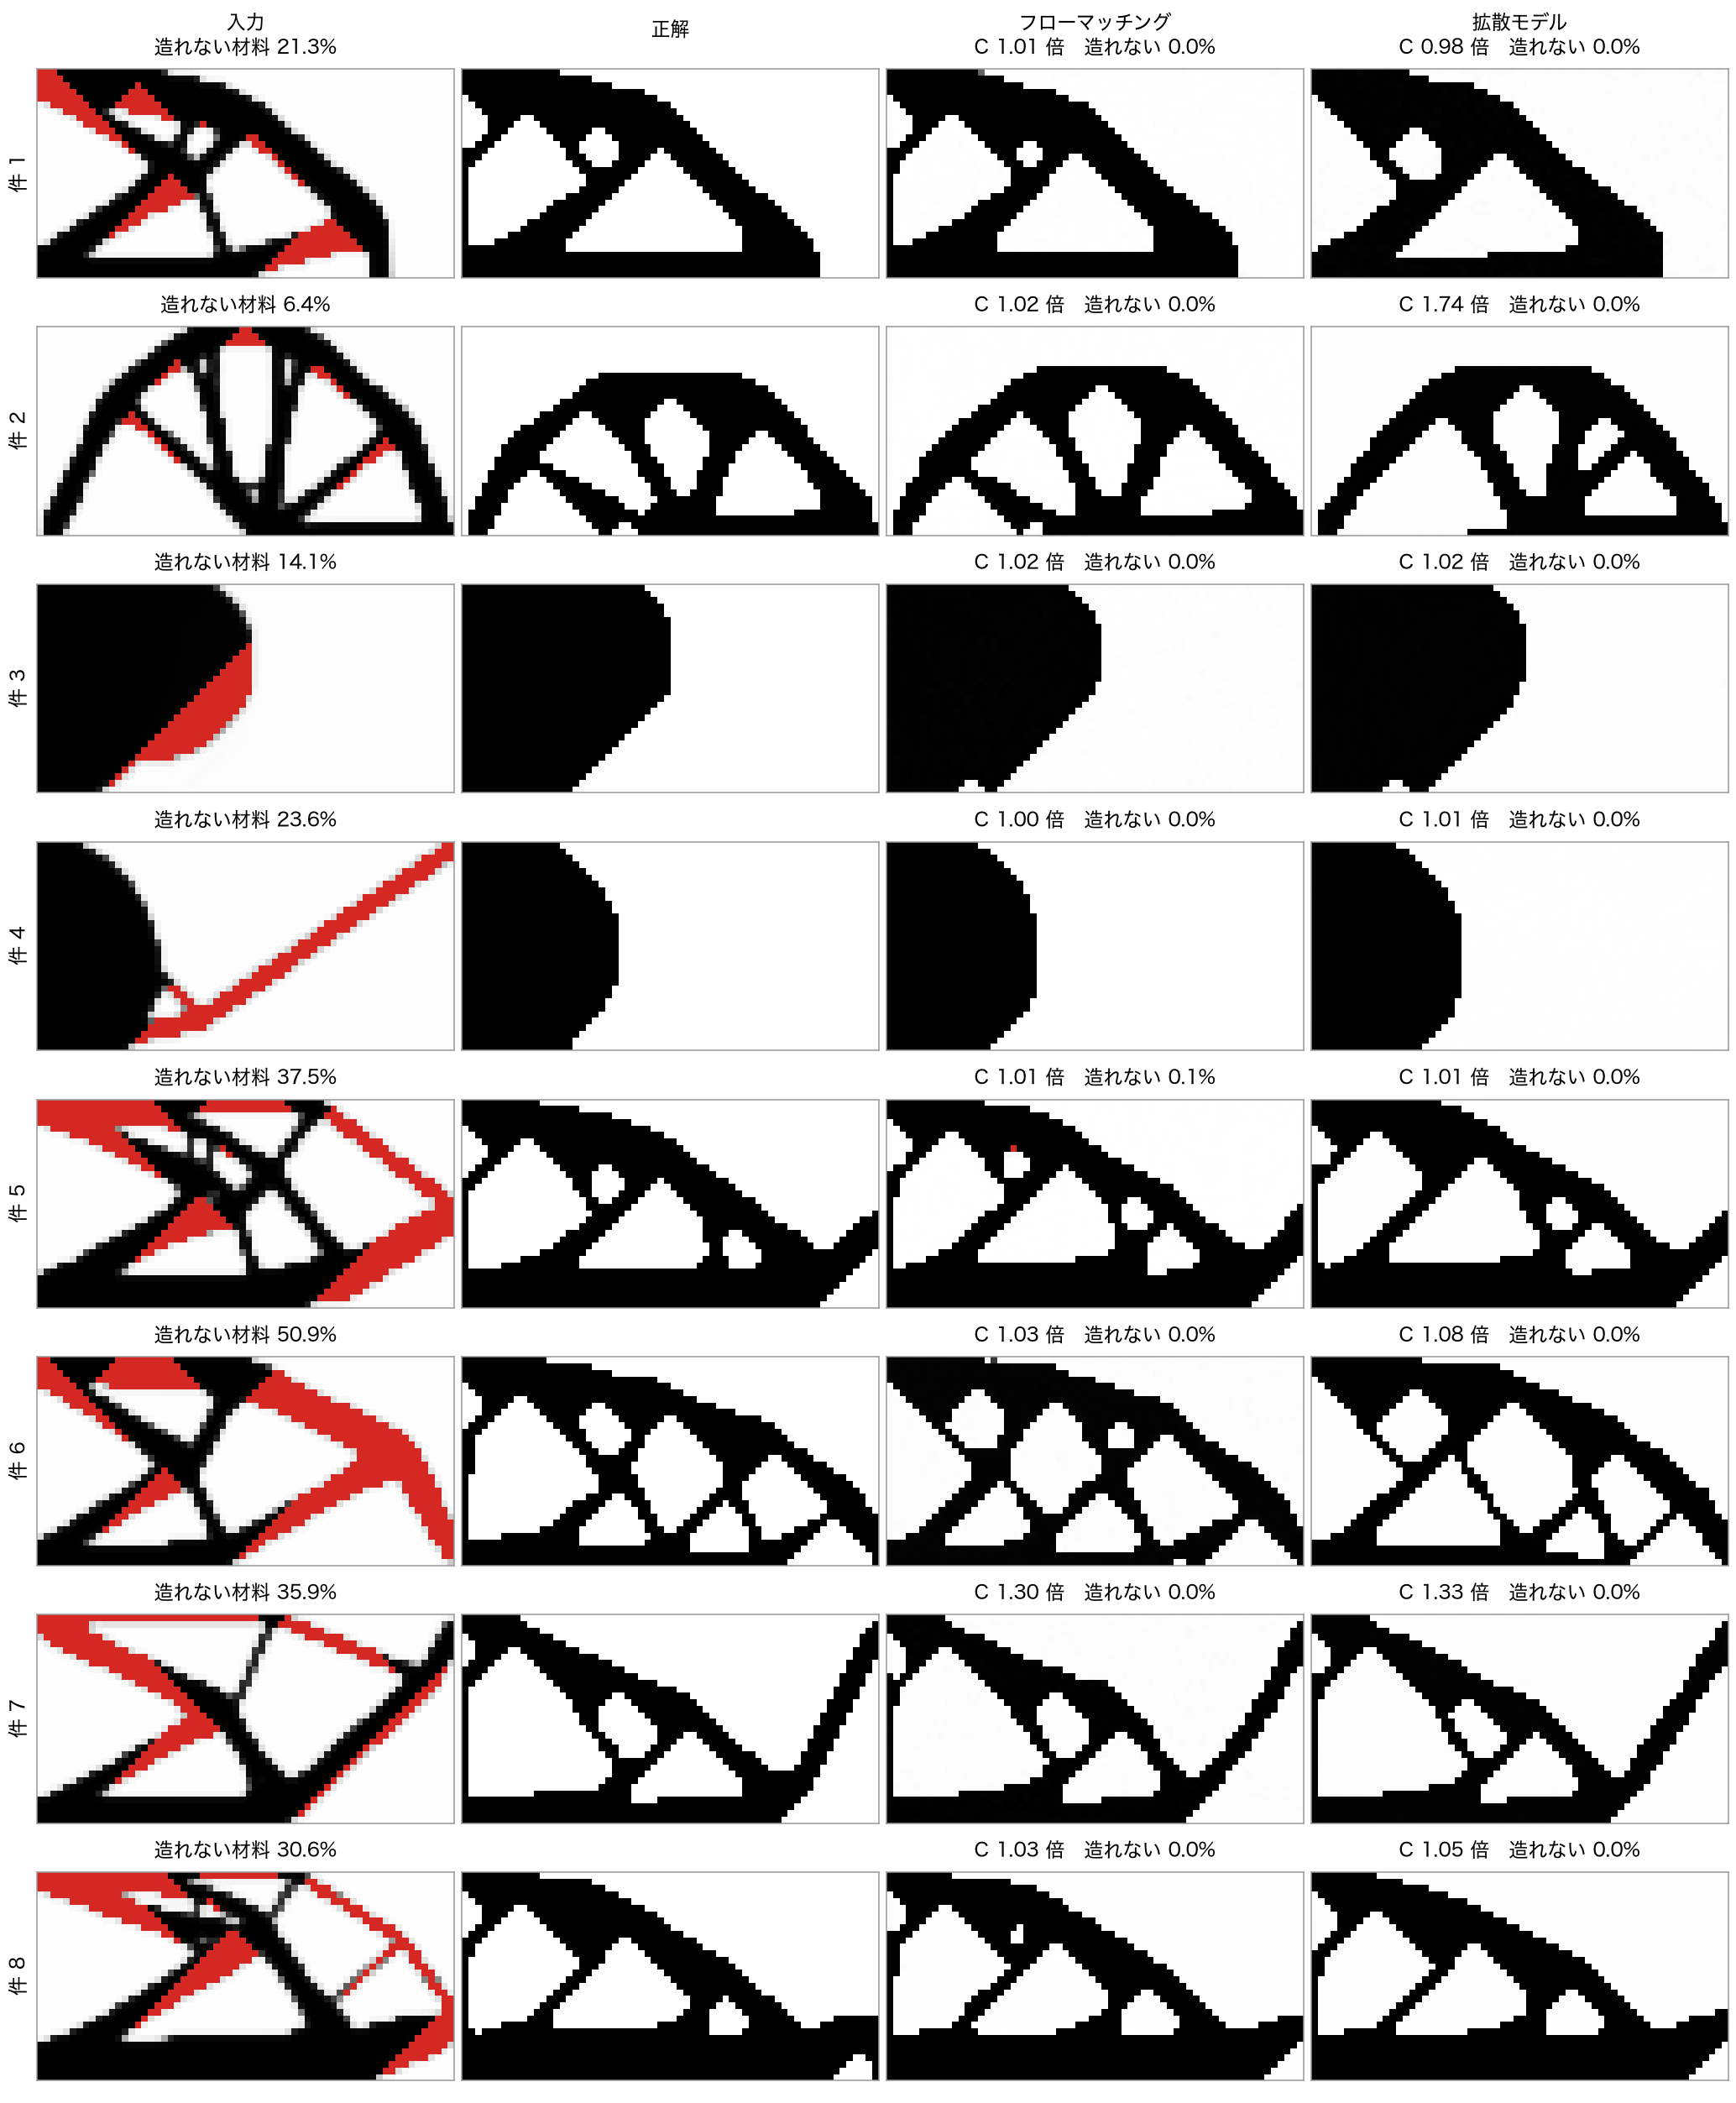
\includegraphics[width=\linewidth]{figs/fig_results.png}
  \caption{単純化した正解で学習したモデルの出力（どのモデルも見ていないテストの先頭 8 件，各モデルの 1 案目）．
           C は正解に対するコンプライアンスの比．赤は造れない材料．}
  \label{fig:results}
\end{figure}

どちらのモデルも，グレーのない単純な形を出力し，穴の数も正解とほぼ同じになった．
今回は，IoU とコンプライアンスの比のどちらもフローマッチングのほうが良かった．
フローマッチングは生成も速いので，今後はフローマッチングを主に使う．

前のモデル（細い部材の多い正解を白黒にして学習したもの）とも比べた．
比べたのは，前と今回のどちらのモデルも学習で見ていない 70 件である．
\begin{itemize}
  \item 浮いた材料のある案：前の拡散・フローは 34\%・33\%，今回の拡散・フローは 7\%・3\%．
  \item 造れない材料のある案：前は 24\%・30\%，今回は 7\%・7\%．
  \item 穴の数の平均：前は 4.3・4.5，今回は 1.7・1.8．
\end{itemize}
正解を単純にしたことで，細い部材と浮いたかけらが大きく減った．

\clearpage
\section{まとめと今後の課題}

\begin{itemize}
  \item JuliaOptopus で free と self の組を作り，トポロジー最適化の結果をオーバーハングのない形に直す生成モデルを学習した．
  \item 5000 件で学習すると，複雑な正解の形もおおむね生成できた
        （コンプライアンスの比 1.024，造れない材料のある案 18\%）．
        ただし，出力にグレーと浮いたかけらが残った．
  \item 正解を大きなフィルター半径と $\beta$ の継続法で解き直して単純にし，白黒にした．
        その結果，グレーのない単純な形を生成できるようになった．
        フローマッチングでは，コンプライアンスの比が 1.011，造れない材料が 1\% を超える案が 3\%，浮いた材料が 1\% を超える案が 0\% である．
\end{itemize}

今後の課題を挙げる．
\begin{itemize}
  \item 荷重の通り道が切れた案（比が 2 倍を超える案）が 2\% ある．
        4 案から有限要素解析で選べば 0\% になるので，複数案から選ぶ使い方が有効である．
  \item わずかに残る造れない材料と浮いた材料は，後処理（ベースプレートから支えられない材料を消す）で取り除ける可能性がある．
  \item 今回は造形方向が上向き，$64 \times 32$ 要素だけである．
        造形方向を変えた場合や，より細かい格子への拡張が必要である．
  \item 左右反転などでデータを増やす（データ拡張）．
\end{itemize}

\end{document}
